\documentclass[a4paper,12pt]{article}
\usepackage[T2A]{fontenc}
\usepackage[utf8]{inputenc}
\usepackage[russian]{babel}
\usepackage{graphicx}
\usepackage{float}
\usepackage{subcaption}
\usepackage{amsmath, amssymb}
\usepackage{geometry}
\usepackage{amsmath}
\usepackage{tikz}
\geometry{top=2cm, bottom=2cm, left=3cm, right=1.5cm}

\begin{document}

\thispagestyle{empty}
\begin{center}
    \large
    Министерство науки и высшего образования Российской Федерации\\
    Федеральное государственное автономное образовательное учреждение\\
    высшего образования\\
    «Национальный исследовательский университет ИТМО»\\
    \vspace{5cm}
    \textbf{Отчёт по исследовательской работе № 1}\\
    \textbf{По предмету: Математический анализ и основы вычислений}\\
    \vspace{6cm}
    \begin{flushright}
        Выполнил работу:\\ Тиганов Вадим Игоревич\\
        \vspace{1cm}
        Академическая группа: \\ J3112\\
        \vspace{1cm}
        Вариант: \\18
    \end{flushright}
    \vspace{1cm}
    \vspace{3cm}
    \begin{center}
        Санкт-Петербург, 2025\\
    \end{center}
\end{center}

\newpage


\section{Ход работы}


\subsection{Задание 3}

Требуется:
\begin{enumerate}
    \item Найти площадь фигуры, заданной параметрически, и нарисовать ее.
\end{enumerate}

\[
x(t) = a \sin(4t)
\]
\[
y(t) = a \sin(t)
\]


\emph{Графическое изображение фигуры:}
\begin{figure}[H]
    \centering
    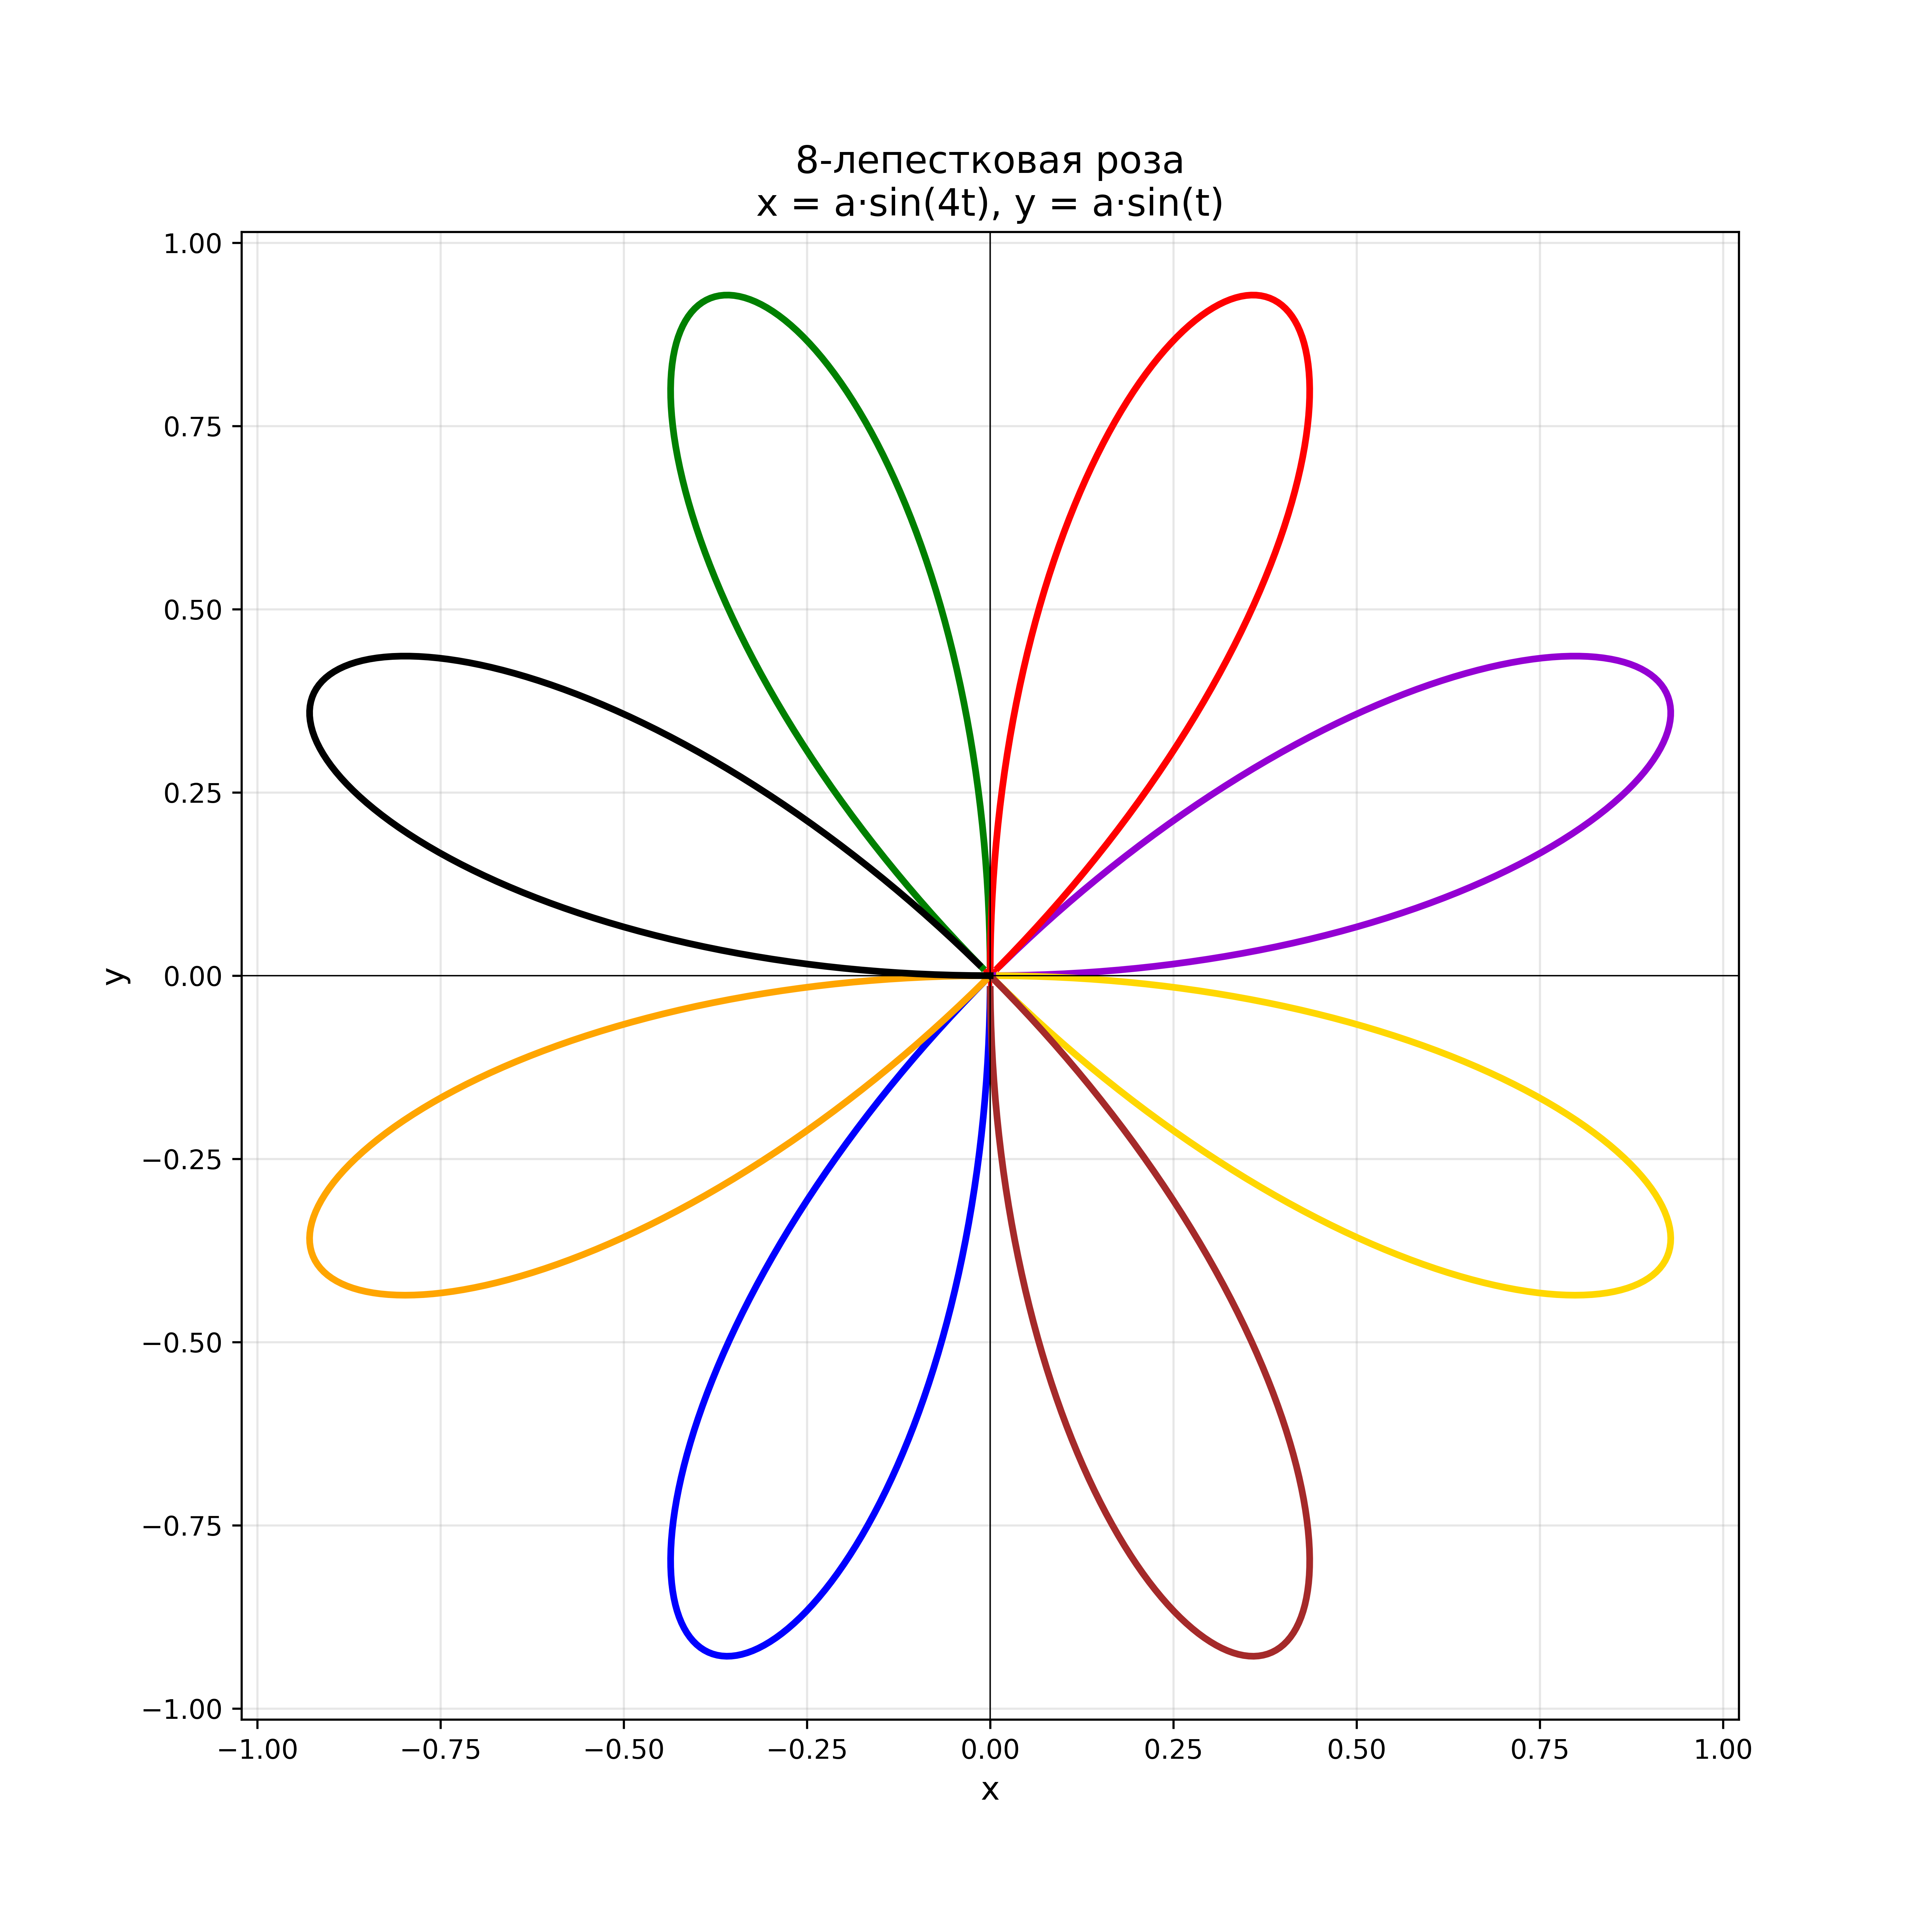
\includegraphics[width=0.9\linewidth]{../img/task3_graph.png}
    \label{fig:integral}
\end{figure}

\emph{Решение задачи:}

\begin{figure}[H]
    \centering
    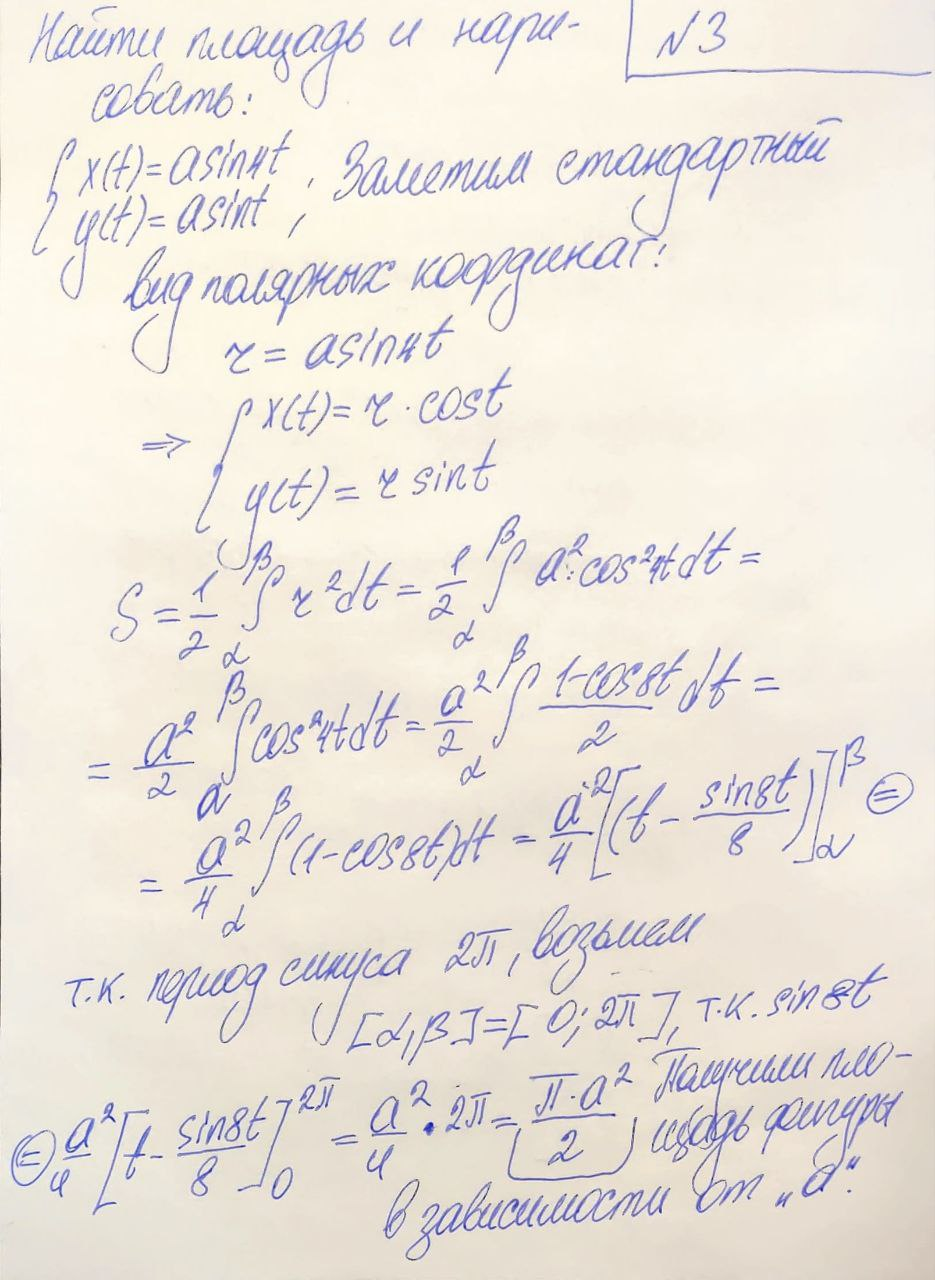
\includegraphics[width=0.8\linewidth]{../img/3_1.jpg}
    \caption{}
    \label{fig:part1}
\end{figure}

\begin{figure}[H]
    \centering
    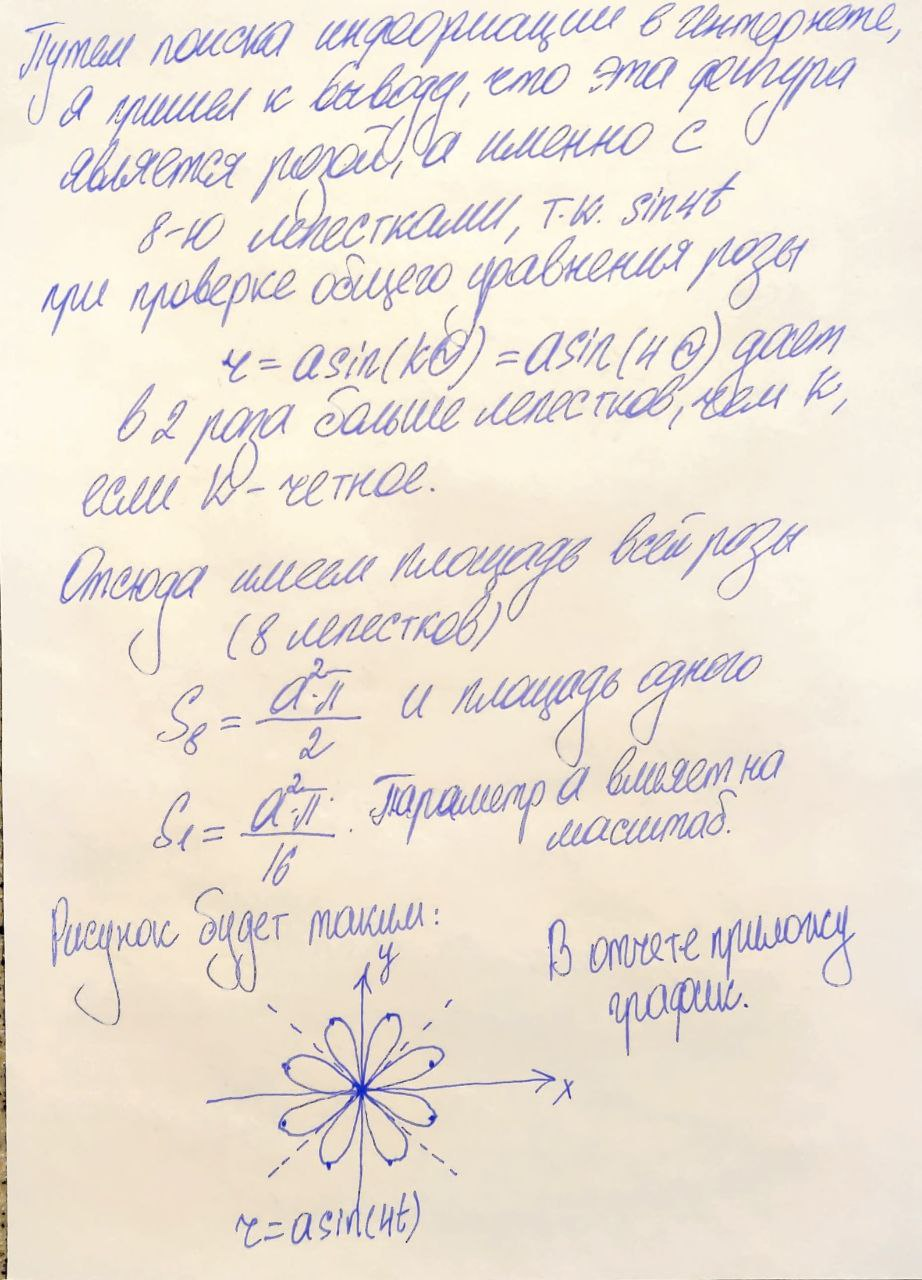
\includegraphics[width=0.8\linewidth]{../img/3_2.jpg}
    \caption{}
    \label{fig:part1}
\end{figure}

\emph{Главная идея - переход в полярные координаты от параметрического уравнения фигуры.}\\
Еще приведу некоторые вычисления площадей для фигуры:\\
\emph{Один лепесток:}
\[
S_1 = \frac{a^2  \pi}{16} = \frac{\pi}{16}
\]
\emph{Вся фигура:}
\[
S_8 = \frac{a^2  \pi}{2} = \frac{\pi}{2}
\]
\emph{Взяв параметр a = 1}

\subsection*{\emph{NB Личные замечания и впечатления от задачи}}
Данная задача \emph{(на момент решения третьего номера)} была самой интересной и 
"математически" красивой. \\
Поискал информацию о розах в интернете, оказалось, что 
они являются одними из самых известных графиков, которые можно построить параметрически 
и в полярных координатах, часто применяются в дизайне. (например, векторная графика для логотипа
цветочного магазина, как я думаю)\\

Некоторые свойства роз:\\

Роза, заданная в полярных координатах, имеет определённое количество лепестков:\\

\( r = a \sin(k \theta) \), то:
\begin{itemize}
    \item если \( k \mod 2 = 0 \), то количество лепестков будет \( 2k \);
    \item если \( k \mod 2 = 1 \), то количество лепестков будет \( k \).
    \item кривая симметрична относительно оси \( y \), так как используется синус;
    \item если \( a \) отрицательно, то лепестки будут направлены в противоположную сторону.
\end{itemize}

\emph{А еще можно нарисовать красивый цветочек, который спасет от отчисления!}
\begin{figure}[H]
    \centering
    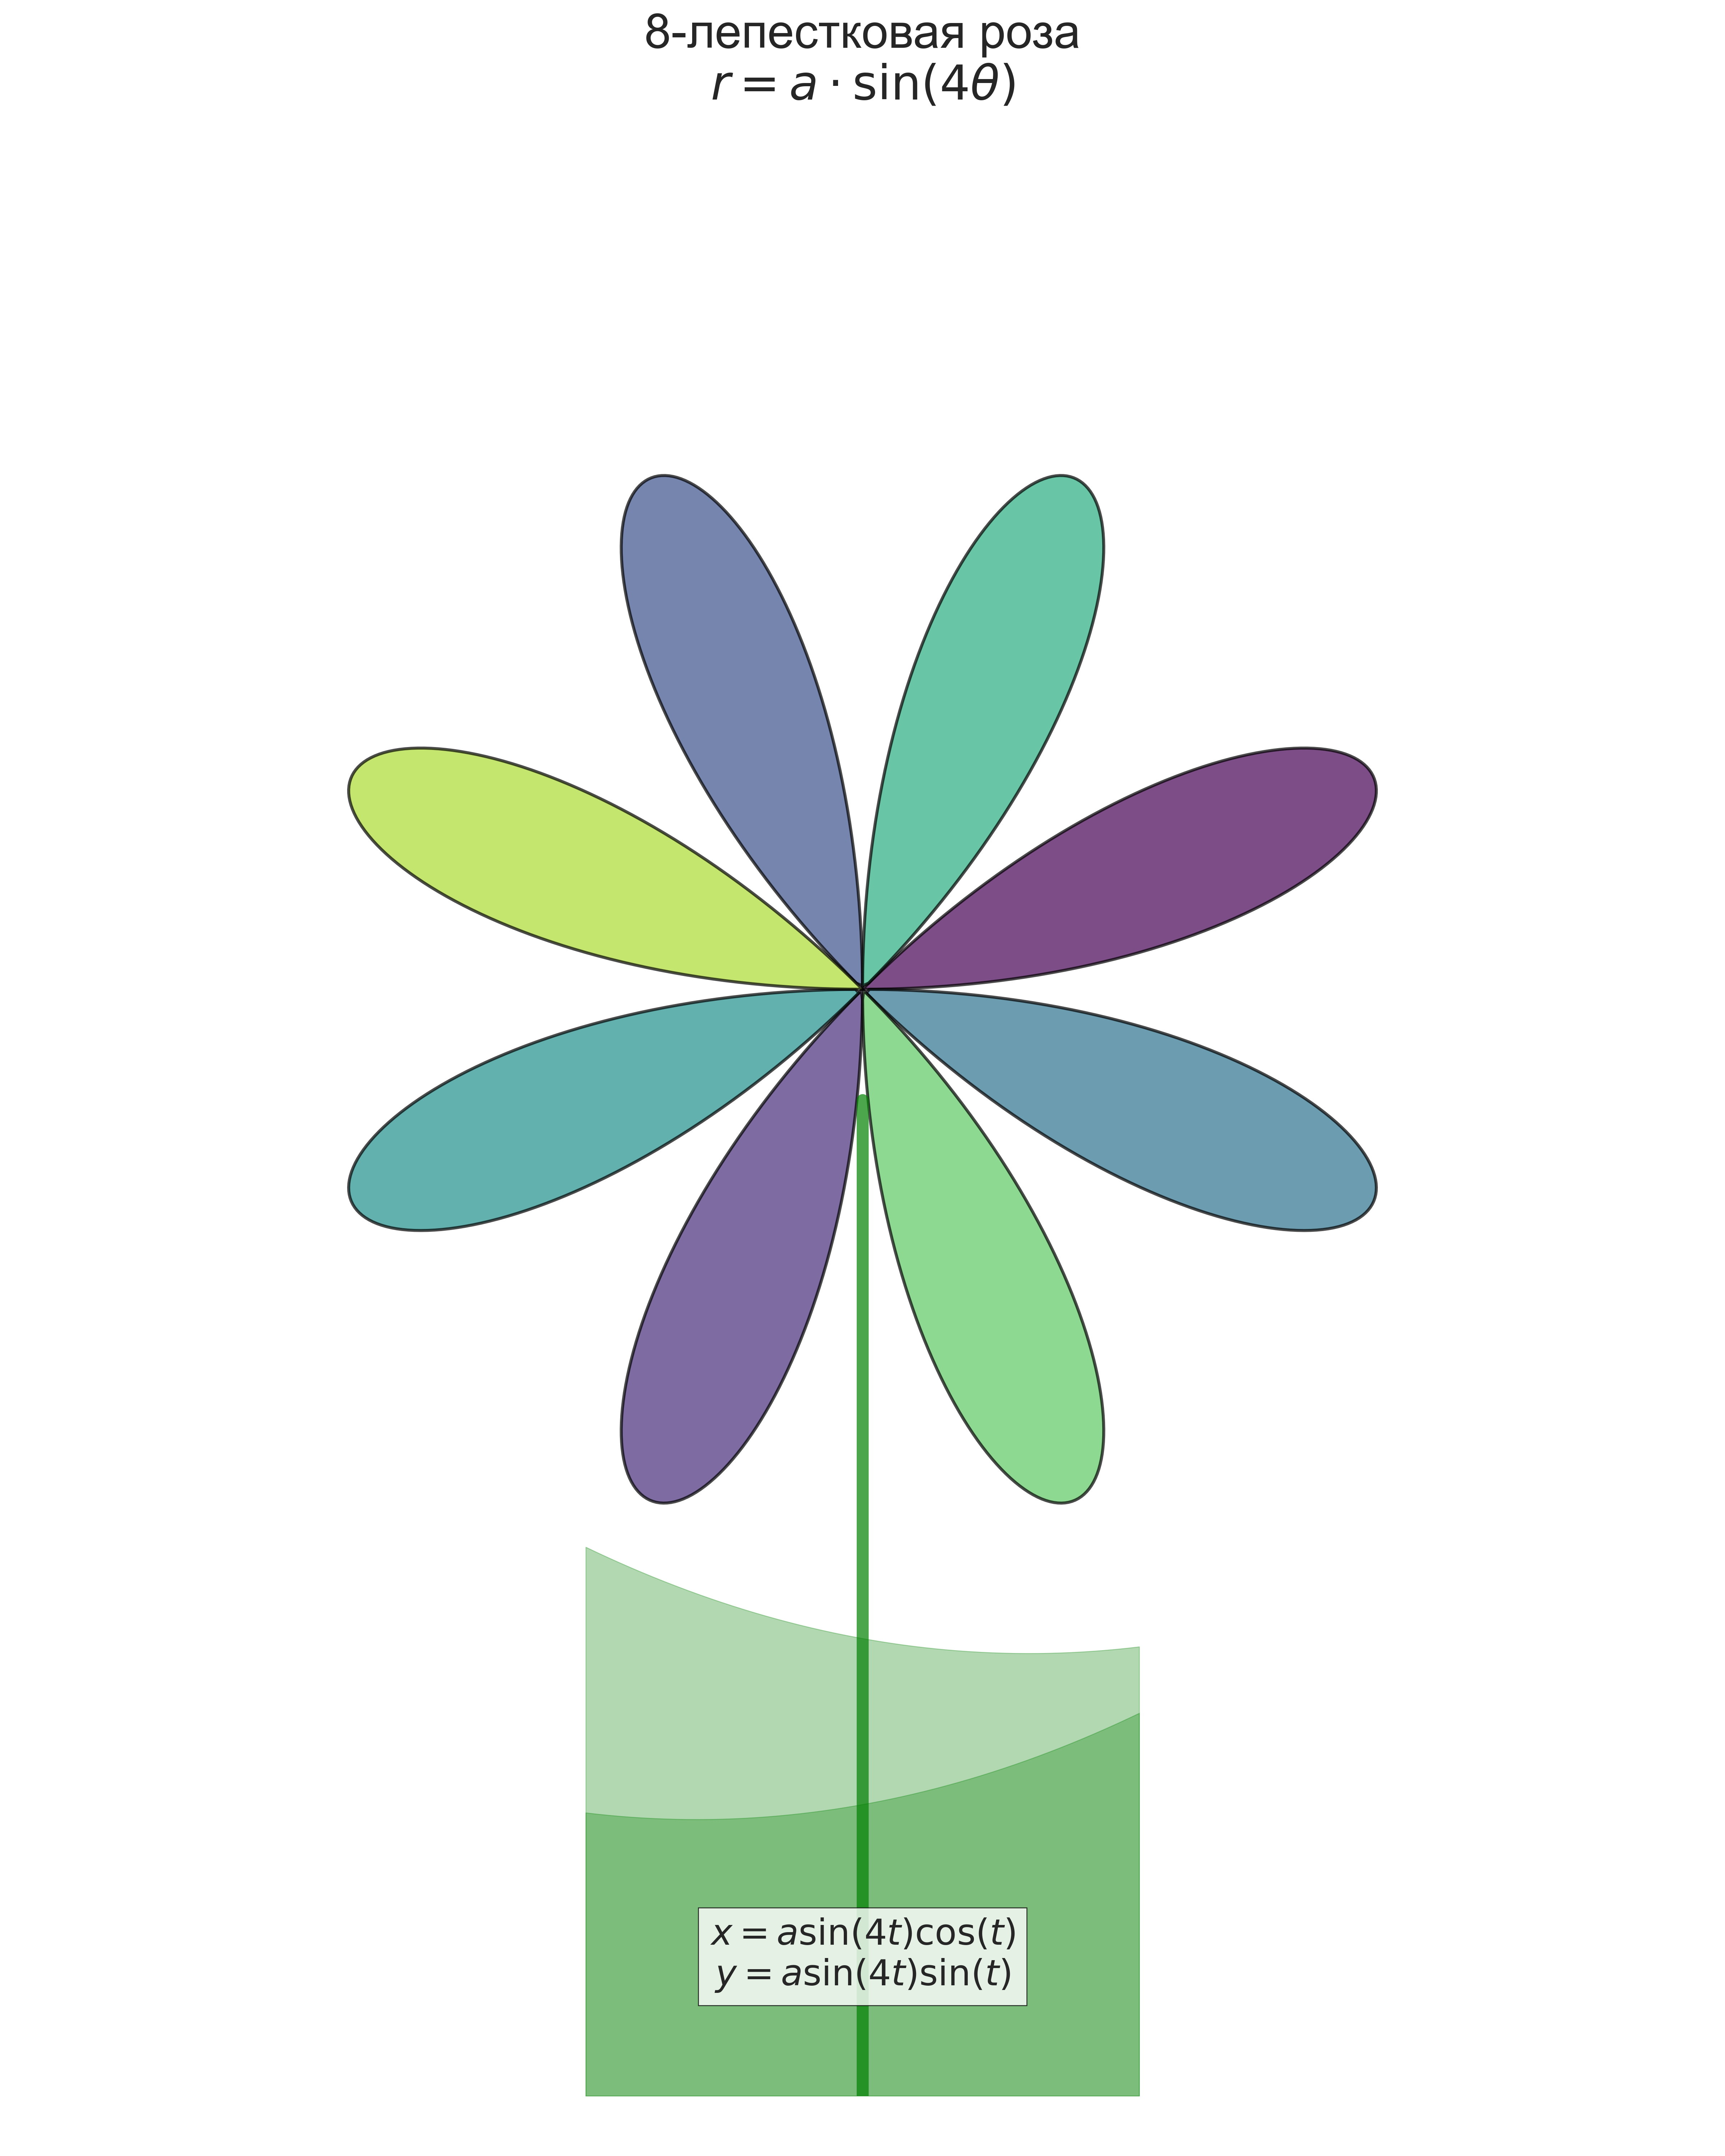
\includegraphics[width=0.5\linewidth]{../img/rose.png}
    \caption{}
    \label{fig:part1}
\end{figure}


\end{document}